% --
% feature selection

\section{Experiments on MFCC Feature Selection}\label{sec:exp_fs}
Feature selection is a very important step prior to neural network training.
A reduction of input features always means a reduction of computations, hence it is a crucial point to evaluate for finding energy efficient models.
Unfortunately it is not always clear which feature are contributing to good classification scores and which do not or even worsen them.
In this section only MFCCs and their enhancements, as described in \rsec{signal_mfcc}, are the focus in the experiments.
A feature selection for raw audio samples, such as used in the Wavenet architecture, would not make any sense, because each sample is a feature itself.
Another important aspect in the feature selection experiments is the evaluation of the proposed frame-based normalization \req{signal_mfcc_norm} originally intended to improve the visualization of MFCCs and making the Generator network of GANs easier and faster to train.
However frame-based normalization might be critical, because this normalization applies only on the frame (time) dimension and disregards the frequency dimension.

Two experiments perform on the MFCC feature selection and evaluates:
\begin{enumerate}
    \item The impact on the amount of cepstral coefficients and
    \item the impact on the enhancements of MFCCs.
\end{enumerate}
For saving training time and computations, those experiments were done on a smaller training set than the whole speech commands dataset, described in \rsec{exp_dataset_speech_cmd}, by using 500 samples of each one of the L12 labels.
The filter bands of the MFCCs were fixed to a total number of 32 bands for all experiments.
Five consecutive training instances perform the training of one set of selected parameters on the same model to create better statistics for the evaluation scores.
The statistics present a mean value and the standard deviation (square root of the variance) of the accuracy scores from all training instances.
The experiments do not apply any early stopping mechanism and therefore use the model parameters from the last epoch for evaluation.
Note that the experiments in this sections are not meant for comparison to the benchmark networks, as described in \rsec{prev_kws_benchmark}, because not the whole dataset was used.


% --
% cepstral

\subsection{Impact on the Amount of Cepstral Coefficients}
The experiment on the impact of the amount of cepstral coefficients evaluates the accuracies of different neural network models using a number of either 12 or 32 cepstral coefficients from the extracted MFCCs.
Note that a number of 12 coefficients with enhancements is commonly applied in many papers.
The experiments were performed once with and once without frame-based normalization to observe its impact on the classification accuracy as well.
Further, the trained models were evaluated regarding their noise and shift invariance, as described in \rsec{exp_details_tb}.
The experiment uses the standard set of training hyperparameters, as listed in \rtab{exp_details_params_train}.
\rtab{exp_fs_cepstral_l12} shows the results of the experiment with 2000 training epochs performed on all three CNN models.
Note that the normalization is active if the table lists \enquote{1} in the \enquote{norm} column, otherwise the normalization is not applied, indicated with \enquote{0}.
\begin{table}[ht!]
\begin{center}
\caption{Experiment on the impact of the amount of cepstral coefficient of MFCC features with additional frame based normalization evaluation.}
\begin{tabular}{ M{3cm}  M{2cm}  M{2cm}  M{2.5cm}  M{2.5cm} }
\toprule
\textbf{arch} & \textbf{mfcc} & \textbf{norm} & \textbf{acc test} & \textbf{acc my} \\
\midrule
conv-trad & mfcc32-12 & 0 & $81.73 \pm 1.58$ & $80.80 \pm 5.88$ \\
conv-trad & mfcc32-12 & 1 & $75.97 \pm 1.15$ & $90.40 \pm 4.80$ \\
conv-trad & mfcc32-32 & 0 & $80.90 \pm 0.81$ & $81.60 \pm 7.84$ \\
conv-trad & mfcc32-32 & 1 & $74.93 \pm 1.09$ & $88.80 \pm 5.31$ \\
\midrule
conv-fstride & mfcc32-12 & 0 & $74.03 \pm 0.87$ & $73.60 \pm 8.62$ \\
conv-fstride & mfcc32-12 & 1 & $66.33 \pm 1.29$ & $79.20 \pm 6.40$ \\
conv-fstride & mfcc32-32 & 0 & $72.07 \pm 2.24$ & $72.80 \pm 8.54$ \\
conv-fstride & mfcc32-32 & 1 & $63.63 \pm 1.15$ & $91.20 \pm 1.60$ \\
\midrule
conv-jim & mfcc32-12 & 0 & $78.73 \pm 1.55$ & $76.00 \pm 6.69$ \\
conv-jim & mfcc32-12 & 1 & $71.77 \pm 1.77$ & $73.60 \pm 5.43$ \\
conv-jim & mfcc32-32 & 0 & $76.43 \pm 1.52$ & $83.20 \pm 2.99$ \\
conv-jim & mfcc32-32 & 1 & $65.73 \pm 1.94$ & $67.20 \pm 6.88$ \\
\bottomrule
\label{tab:exp_fs_cepstral_l12}
\end{tabular}
\end{center}
\end{table}
\FloatBarrier
\noindent
\rfig{exp_fs_cepstral_acc} shows the accuracies on the validation set of the best performing training instances for each model, where the accuracies are smoothed by a striding average filter with a length of 10 epochs for better visualization.
\begin{figure}[!ht]
  \centering
  \subfigure[conv-trad]{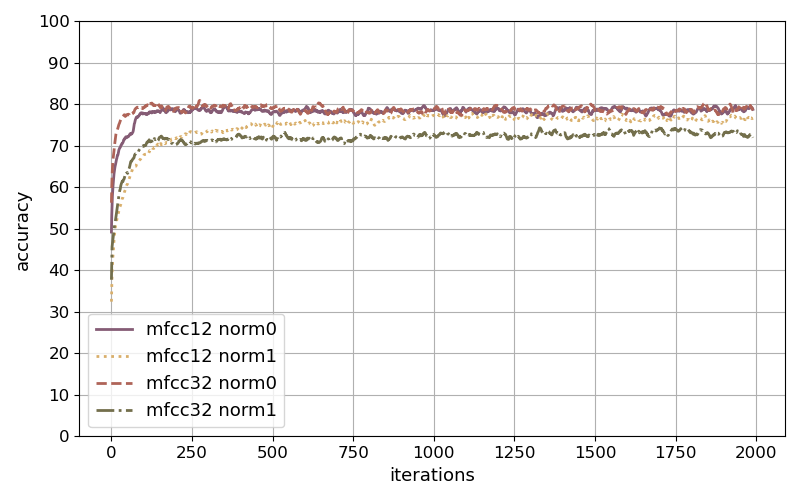
\includegraphics[width=0.45\textwidth]{./5_exp/figs/exp_fs_cepstral_acc_conv-trad.png}}
  \subfigure[conv-fstride]{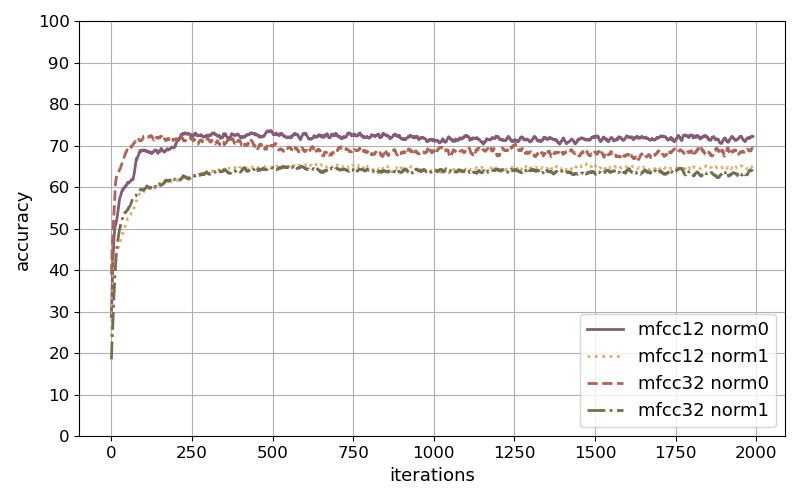
\includegraphics[width=0.45\textwidth]{./5_exp/figs/exp_fs_cepstral_acc_conv-fstride.png}}
  \subfigure[conv-jim]{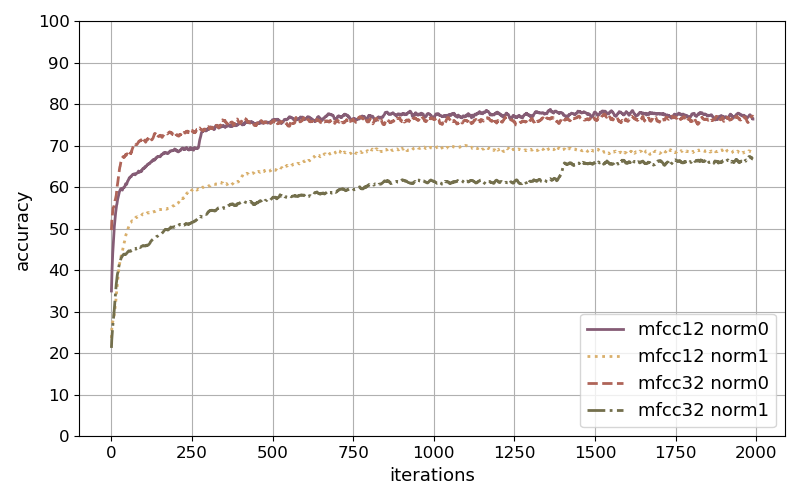
\includegraphics[width=0.45\textwidth]{./5_exp/figs/exp_fs_cepstral_acc_conv-jim.png}}
  \caption{Accuracies on the validation set of all three CNN models of their best training instance, with different amounts of cepstral coefficients and with and without frame-based normalization. Applied smoothing with a 10 epoch average filter.}
  \label{fig:exp_fs_cepstral_acc}
\end{figure}
\FloatBarrier
\noindent
From the provided results it can be observed that the usage of 32 cepstral coefficients does not improve the accuracies compared to the 12 coefficients.
Also the overfitting effects are more prominent with 32 coefficients.
Further they show that frame-based normalization usually achieves less accuracy and requires more epochs until convergence is reached.

In the following the shift and noise invariance of each model is evaluated.
The noise and shift invariance of the \texttt{conv-trad} model is shown in \rfig{exp_fs_cepstral_tb_noise_conv-trad} and \rfig{exp_fs_cepstral_tb_shift_conv-trad} respectively.
\begin{figure}[!ht]
  \centering
  \subfigure[mfcc12, norm0]{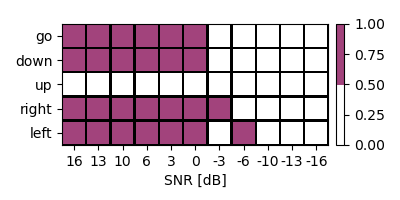
\includegraphics[width=0.35\textwidth]{./5_exp/figs/exp_fs_cepstral_tb_noise_conv-trad_mfcc12_norm0.png}}
  \subfigure[mfcc12, norm1]{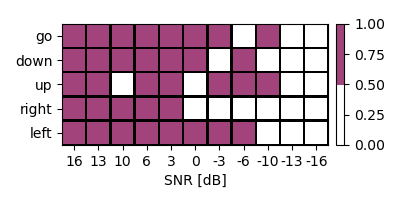
\includegraphics[width=0.35\textwidth]{./5_exp/figs/exp_fs_cepstral_tb_noise_conv-trad_mfcc12_norm1.png}}
  \subfigure[mfcc32, norm0]{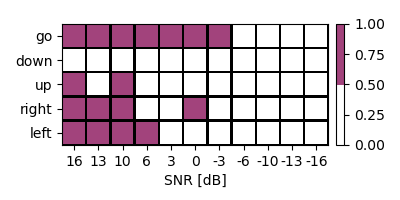
\includegraphics[width=0.35\textwidth]{./5_exp/figs/exp_fs_cepstral_tb_noise_conv-trad_mfcc32_norm0.png}}
  \subfigure[mfcc32, norm1]{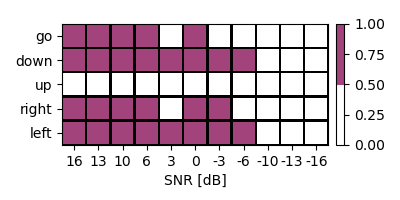
\includegraphics[width=0.35\textwidth]{./5_exp/figs/exp_fs_cepstral_tb_noise_conv-trad_mfcc32_norm1.png}}
  \caption{Noise invariance of the \texttt{conv-trad} model, with different amounts of cepstral coefficients and with and without frame-based normalization.}
  \label{fig:exp_fs_cepstral_tb_noise_conv-trad}
\end{figure}
\FloatBarrier
\noindent
\begin{figure}[!ht]
  \centering
  \subfigure[mfcc12, norm0]{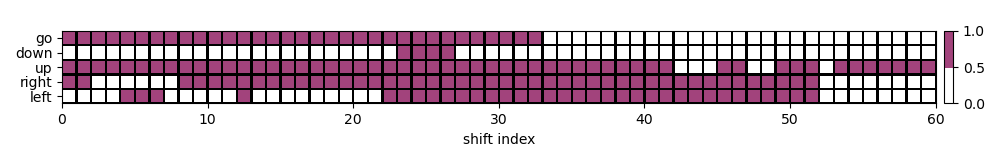
\includegraphics[width=0.45\textwidth]{./5_exp/figs/exp_fs_cepstral_tb_shift_conv-trad_mfcc12_norm0.png}}
  \subfigure[mfcc12, norm1]{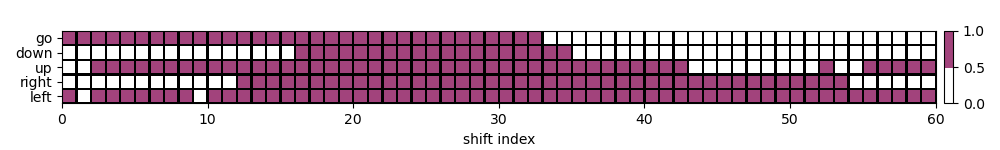
\includegraphics[width=0.45\textwidth]{./5_exp/figs/exp_fs_cepstral_tb_shift_conv-trad_mfcc12_norm1.png}}
  \subfigure[mfcc32, norm0]{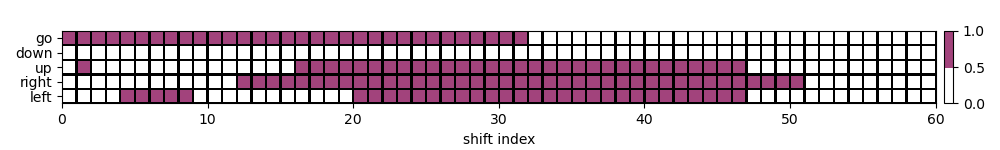
\includegraphics[width=0.45\textwidth]{./5_exp/figs/exp_fs_cepstral_tb_shift_conv-trad_mfcc32_norm0.png}}
  \subfigure[mfcc32, norm1]{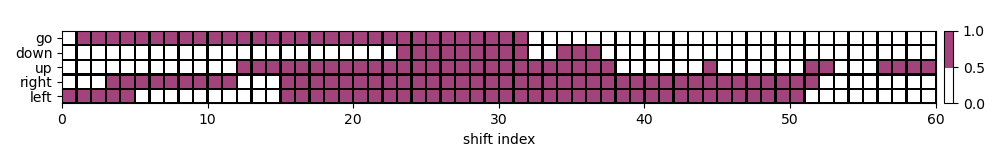
\includegraphics[width=0.45\textwidth]{./5_exp/figs/exp_fs_cepstral_tb_shift_conv-trad_mfcc32_norm1.png}}
  \caption{Shift invariance of the \texttt{conv-trad} model, with different amounts of cepstral coefficients and with and without frame-based normalization.}
  \label{fig:exp_fs_cepstral_tb_shift_conv-trad}
\end{figure}
\FloatBarrier
\noindent
The noise and shift invariance of the \texttt{conv-fstride} model is shown in \rfig{exp_fs_cepstral_tb_noise_conv-fstride} and \rfig{exp_fs_cepstral_tb_shift_conv-fstride} respectively.
\begin{figure}[!ht]
  \centering
  \subfigure[mfcc12, norm0]{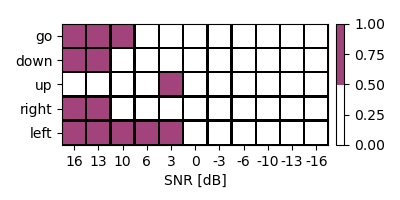
\includegraphics[width=0.35\textwidth]{./5_exp/figs/exp_fs_cepstral_tb_noise_conv-fstride_mfcc12_norm0.png}}
  \subfigure[mfcc12, norm1]{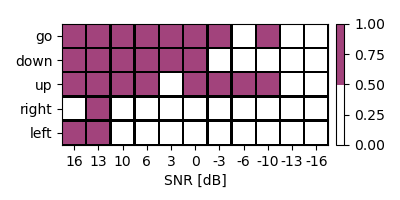
\includegraphics[width=0.35\textwidth]{./5_exp/figs/exp_fs_cepstral_tb_noise_conv-fstride_mfcc12_norm1.png}}
  \subfigure[mfcc32, norm0]{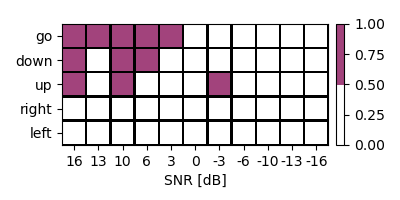
\includegraphics[width=0.35\textwidth]{./5_exp/figs/exp_fs_cepstral_tb_noise_conv-fstride_mfcc32_norm0.png}}
  \subfigure[mfcc32, norm1]{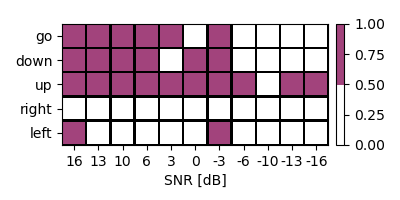
\includegraphics[width=0.35\textwidth]{./5_exp/figs/exp_fs_cepstral_tb_noise_conv-fstride_mfcc32_norm1.png}}
  \caption{Noise invariance of the \texttt{conv-fstride} model, with different amounts of cepstral coefficients and with and without frame-based normalization.}
  \label{fig:exp_fs_cepstral_tb_noise_conv-fstride}
\end{figure}
\FloatBarrier
\noindent
\begin{figure}[!ht]
  \centering
  \subfigure[mfcc12, norm0]{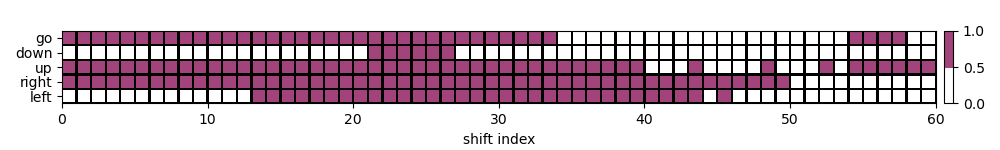
\includegraphics[width=0.45\textwidth]{./5_exp/figs/exp_fs_cepstral_tb_shift_conv-fstride_mfcc12_norm0.png}}
  \subfigure[mfcc12, norm1]{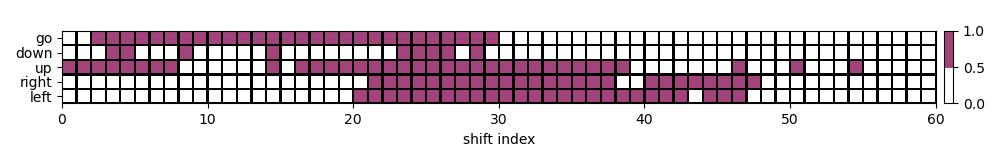
\includegraphics[width=0.45\textwidth]{./5_exp/figs/exp_fs_cepstral_tb_shift_conv-fstride_mfcc12_norm1.png}}
  \subfigure[mfcc32, norm0]{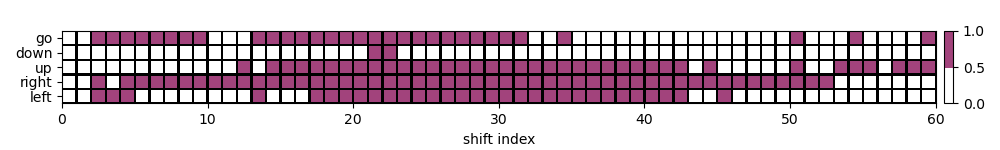
\includegraphics[width=0.45\textwidth]{./5_exp/figs/exp_fs_cepstral_tb_shift_conv-fstride_mfcc32_norm0.png}}
  \subfigure[mfcc32, norm1]{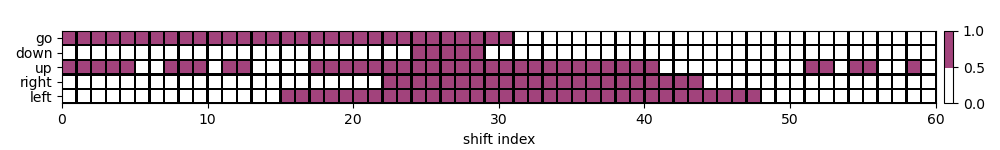
\includegraphics[width=0.45\textwidth]{./5_exp/figs/exp_fs_cepstral_tb_shift_conv-fstride_mfcc32_norm1.png}}
  \caption{Shift invariance of the \texttt{conv-fstride} model, with different amounts of cepstral coefficients and with and without frame-based normalization.}
  \label{fig:exp_fs_cepstral_tb_shift_conv-fstride}
\end{figure}
\FloatBarrier
\noindent
The noise and shift invariance of the \texttt{conv-jim} model is shown in \rfig{exp_fs_cepstral_tb_noise_conv-jim} and \rfig{exp_fs_cepstral_tb_shift_conv-jim} respectively.
\begin{figure}[!ht]
  \centering
  \subfigure[mfcc12, norm0]{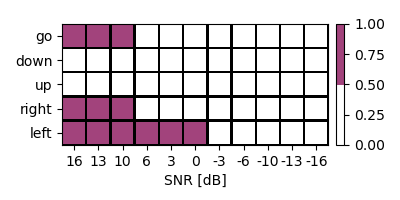
\includegraphics[width=0.35\textwidth]{./5_exp/figs/exp_fs_cepstral_tb_noise_conv-jim_mfcc12_norm0.png}}
  \subfigure[mfcc12, norm1]{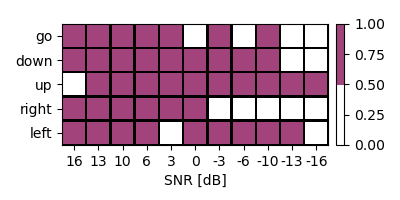
\includegraphics[width=0.35\textwidth]{./5_exp/figs/exp_fs_cepstral_tb_noise_conv-jim_mfcc12_norm1.png}}
  \subfigure[mfcc32, norm0]{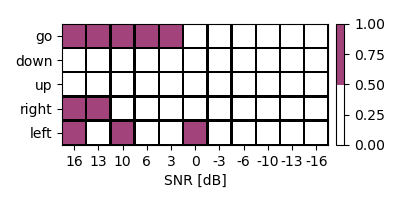
\includegraphics[width=0.35\textwidth]{./5_exp/figs/exp_fs_cepstral_tb_noise_conv-jim_mfcc32_norm0.png}}
  \subfigure[mfcc32, norm1]{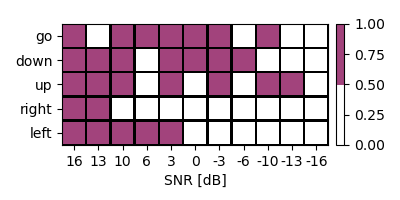
\includegraphics[width=0.35\textwidth]{./5_exp/figs/exp_fs_cepstral_tb_noise_conv-jim_mfcc32_norm1.png}}
  \caption{Noise invariance of the \texttt{conv-jim} model, with different amounts of cepstral coefficients and with and without frame-based normalization.}
  \label{fig:exp_fs_cepstral_tb_noise_conv-jim}
\end{figure}
\FloatBarrier
\noindent
\begin{figure}[!ht]
  \centering
  \subfigure[mfcc12, norm0]{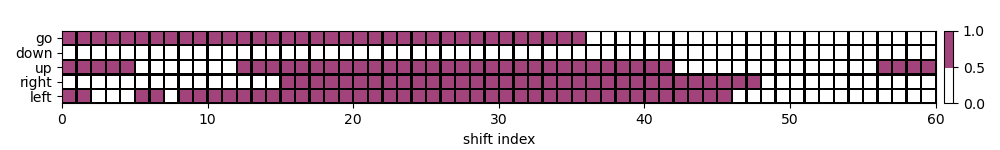
\includegraphics[width=0.45\textwidth]{./5_exp/figs/exp_fs_cepstral_tb_shift_conv-jim_mfcc12_norm0.png}}
  \subfigure[mfcc12, norm1]{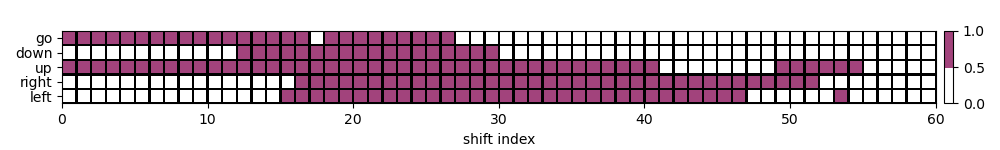
\includegraphics[width=0.45\textwidth]{./5_exp/figs/exp_fs_cepstral_tb_shift_conv-jim_mfcc12_norm1.png}}
  \subfigure[mfcc32, norm0]{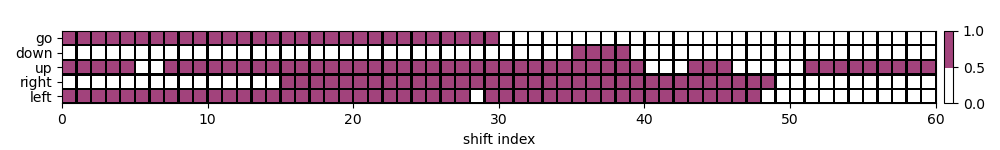
\includegraphics[width=0.45\textwidth]{./5_exp/figs/exp_fs_cepstral_tb_shift_conv-jim_mfcc32_norm0.png}}
  \subfigure[mfcc32, norm1]{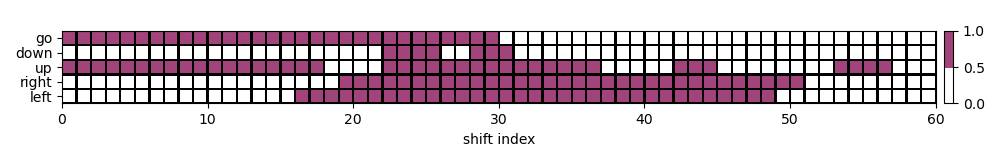
\includegraphics[width=0.45\textwidth]{./5_exp/figs/exp_fs_cepstral_tb_shift_conv-jim_mfcc32_norm1.png}}
  \caption{Shift invariance of the \texttt{conv-jim} model, with different amounts of cepstral coefficients and with and without frame-based normalization.}
  \label{fig:exp_fs_cepstral_tb_shift_conv-jim}
\end{figure}
\FloatBarrier
\noindent
While the results of the invariance tests do not allow a general conclusion, following patterns can be observed regardless:
The frame-based normalization does certainly increase the invariance in noise, which is logical because the model has to focus more on learning patterns of the individual key words and is less prone to overfitting.
The \texttt{conv-fstride} model does unexpectedly well upon the shift invariance test, even though its strides perform merely on the frequency axis.
However it usually does not achieve that good shift invariance results compared to the other models, and often holes appear in the classification with the shift invariance test.
The \texttt{conv-trad} performs best on all tests, but also requires a higher computational footprint, so that the preferred model is \texttt{conv-jim} with a good trade-off between computational footprint and classification results.
The usage of 32 MFCC coefficients does not improve the invariance against shift or noise and very often worsens the results.


% --
% enhancements

\subsection{Impact on the Enhancements of MFCCs}\label{sec:exp_fs_mfcc}
In this experiment the cepstral coefficients were selected to 12 and enhanced with deltas, double deltas and energy vectors, as described in \rsec{signal_mfcc_enhancement}.
\rtab{exp_fs_mfcc_l12} lists the results of the experiments with applied frame-based normalization, 2000 training epochs and the standard hyperparameters for CNN models.
Note that a \enquote{1}, in the columns for the enhancements, means that a specific enhancement is included, otherwise it is denoted as \enquote{0}. 
\begin{table}[ht!]
\small
\begin{center}
\caption{Experiment on the impact of feature enhancement of cepstral coefficients (c), deltas (d), double deltas (dd) and energy vectors (e) performed on the \texttt{conv-jim} model with frame-based normalization}
\begin{tabular}{ M{1cm}  M{1cm}  M{1cm}  M{1cm}  M{2.5cm}  M{2.5cm} }
\toprule
\textbf{c} & \textbf{d} & \textbf{dd} & \textbf{e} & \textbf{acc test} & \textbf{acc my} \\
\midrule
0 & 0 & 1 & 0 & $37.40 \pm 2.17$ & $34.40 \pm 11.20$ \\
0 & 0 & 1 & 1 & $46.63 \pm 2.87$ & $36.80 \pm 7.76$ \\
0 & 1 & 0 & 0 & $58.57 \pm 2.06$ & $64.80 \pm 4.66$ \\
0 & 1 & 0 & 1 & $62.00 \pm 1.82$ & $75.20 \pm 11.14$ \\
0 & 1 & 1 & 0 & $59.03 \pm 1.77$ & $56.00 \pm 9.47$ \\
0 & 1 & 1 & 1 & $61.60 \pm 2.28$ & $62.40 \pm 6.97$ \\
1 & 0 & 0 & 0 & $72.00 \pm 1.46$ & $85.60 \pm 1.96$ \\
1 & 0 & 0 & 1 & $72.83 \pm 1.22$ & $80.00 \pm 4.38$ \\
1 & 0 & 1 & 0 & $70.63 \pm 2.13$ & $84.00 \pm 8.76$ \\
1 & 0 & 1 & 1 & $72.36 \pm 2.27$ & $80.00 \pm 4.38$ \\
1 & 1 & 0 & 0 & $72.80 \pm 2.90$ & $88.80 \pm 6.88$ \\
1 & 1 & 0 & 1 & $75.30 \pm 1.38$ & $92.00 \pm 2.53$ \\
1 & 1 & 1 & 0 & $73.43 \pm 2.05$ & $84.80 \pm 5.88$ \\
1 & 1 & 1 & 1 & $73.73 \pm 1.66$ & $83.20 \pm 6.88$ \\
\bottomrule
\label{tab:exp_fs_mfcc_l12}
\end{tabular}
\end{center}
\vspace{-4mm}
\end{table}
\FloatBarrier
\noindent
The best two feature enhancements were the full MFCC-39 features (c1d1d1e1) and the (c1d1d0e1) features without double deltas.
Those were used for examining the accuracy on the validation set during training shown in \rfig{exp_fs_mfcc_tb_acc_conv-jim} and the noise and shift invariance in \rfig{exp_fs_mfcc_tb_noise_conv-jim} and \rfig{exp_fs_mfcc_tb_shift_conv-jim}.
\begin{figure}[!ht]
  \centering
  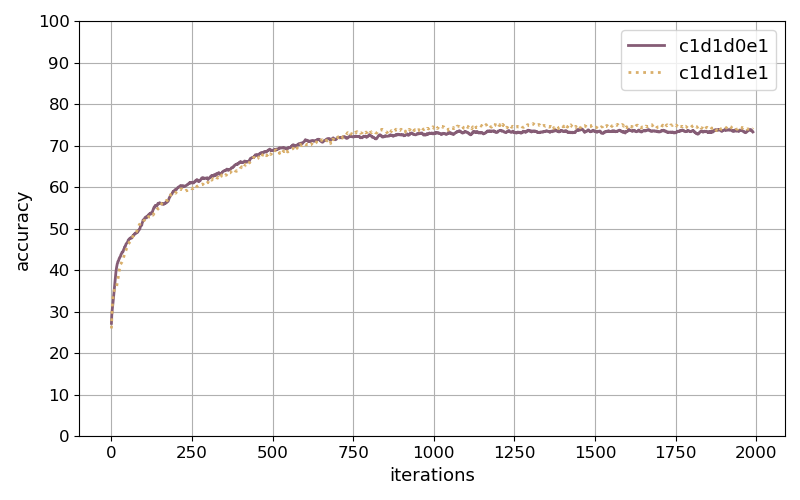
\includegraphics[width=0.45\textwidth]{./5_exp/figs/exp_fs_mfcc_acc_conv-jim.png}
  \caption{Accuracies of the \texttt{conv-jim} model with different feature enhancements and frame-based normalization.}
  \label{fig:exp_fs_mfcc_tb_acc_conv-jim}
\end{figure}
\FloatBarrier
\noindent
\begin{figure}[!ht]
  \centering
  \subfigure[c1d1d1e1]{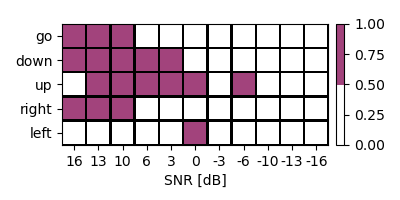
\includegraphics[width=0.35\textwidth]{./5_exp/figs/exp_fs_mfcc_tb_noise_conv-jim_c1d1d1e1.png}}
  \subfigure[c1d1d0e1]{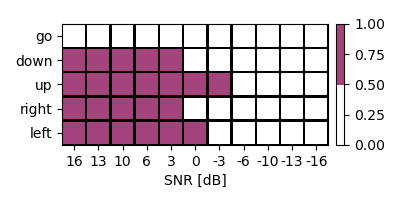
\includegraphics[width=0.35\textwidth]{./5_exp/figs/exp_fs_mfcc_tb_noise_conv-jim_c1d1d0e1.png}}
  \caption{Noise invariance of the \texttt{conv-jim} model with different feature enhancements and frame-based normalization.}
  \label{fig:exp_fs_mfcc_tb_noise_conv-jim}
\end{figure}
\FloatBarrier
\noindent
\begin{figure}[!ht]
  \centering
  \subfigure[c1d1d1e1]{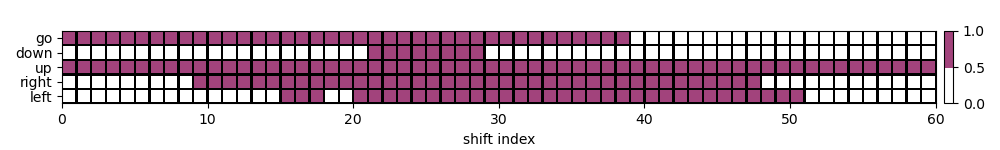
\includegraphics[width=0.45\textwidth]{./5_exp/figs/exp_fs_mfcc_tb_shift_conv-jim_c1d1d1e1.png}}
  \subfigure[c1d1d0e1]{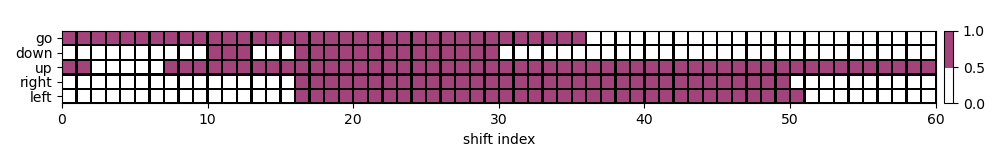
\includegraphics[width=0.45\textwidth]{./5_exp/figs/exp_fs_mfcc_tb_shift_conv-jim_c1d1d0e1.png}}
  \caption{Shift invariance of the \texttt{conv-jim} model with different feature enhancements and frame-based normalization.}
  \label{fig:exp_fs_mfcc_tb_shift_conv-jim}
\end{figure}
\FloatBarrier
\noindent
The experiments show that the enhancements of the MFCC features can improve the classification results significantly, but it also increased the amount of computations for each model.